\section{Real-weight signed kernels and a sharp measure threshold}
\label{real:sec:kernels}

The signed-kernel chapter of the pinned manuscript proves that the strict
depth-two coefficients $H_{n-1}^{(b)}/n^a$, with integer $a\geq1$ and real
$b>0$, have an integrable density with one sign change. That structure
gives a unique zero of the imaginary part on the upper semicircle.
The affine signed-moment continuation already permits real $a\geq1$
for measure existence and total-variation estimates, but does not extend
the one-crossing theorem to that range or treat $0<a<1$~\cite{ProveIt}.
We now classify the complete domain of finite signed measures for these
coefficients. Its boundary has a positive endpoint atom, and requires a
different cancellation argument from the interior.

Hausdorff--Stieltjes methods for polylogarithmic geometry have substantial
existing context. In particular, Li's recent work treats positive
Hausdorff measures and likelihood-ratio ordering for integer-index
multiple \emph{star} polylogarithms~\cite{Li2026}. Here the strict
depth-two sequence has total moment mass zero, so its representing
measure is signed. The results below concern real exponents, the sharp
boundary of finite-measure representability, and the associated zero
arc. The claim of extension is relative to the pinned manuscript; no
complete priority claim is intended.

For $a,b>0$ define
\begin{equation}\label{real:eq:def}
 m_n(a,b)=\frac{H_{n-1}^{(b)}}{n^a},\qquad
 H_{n-1}^{(b)}=\sum_{j=1}^{n-1}j^{-b},\qquad
 F_{a,b}(z)=\sum_{n\geq1}m_n(a,b)z^n\quad(|z|<1).
\end{equation}
The empty harmonic sum is zero. At integer exponents $F_{a,b}$ is the
strict depth-two polylogarithm used in the source manuscript.

\subsection{A real-order kernel with cancellation retained}

For $T>0$ put
\begin{equation}\label{real:eq:kernel}
\begin{split}
 k_{a,b}(T)={}&-\frac{T^{a+b-1}}{\Gamma(a+b)}\\
 &+\frac1{\Gamma(a)\Gamma(b)}
  \int_0^\infty\frac{v^{b-1}}{e^v-1}
    \bigl[T^{a-1}-(T-v)_+^{a-1}\bigr]\,dv,
\end{split}
\end{equation}
and $\kappa_{a,b}(u)=k_{a,b}(-\log u)$ for $0<u<1$.
Here $(T-v)_+^{a-1}$ means $(T-v)^{a-1}$ when $v<T$, and zero when
$v>T$; its value at $v=T$ is irrelevant. In particular, if $0<a<1$,
the left-hand singularity at $v=T$ is retained. The integral converges
absolutely for each fixed $T$: its bracket is $O_T(v)$ at zero, the
singularity at $v=T$ has integrable exponent $a-1>-1$, and the tail
decays exponentially. For $b\leq1$ the two terms inside the bracket
must remain combined near $v=0$.

\begin{theorem}[Sharp finite signed-measure classification]
\label{real:thm:measure}
Let $a,b>0$. There is a finite signed Borel measure $\mu_{a,b}$ on
$[0,1]$ satisfying
\begin{equation}\label{real:eq:moments}
 \int_{[0,1]}u^{n-1}\,d\mu_{a,b}(u)=m_n(a,b),\qquad n\geq1,
\end{equation}
if and only if $a+b\geq1$. Whenever it exists, it is unique and has
total mass zero. More precisely:
\begin{enumerate}
\item If $a+b>1$, the measure is
$d\mu_{a,b}(u)=\kappa_{a,b}(u)\,du$, with $\kappa_{a,b}\in L^1(0,1)$.
There is a unique $r_{a,b}\in(0,1)$ such that
\begin{equation}\label{real:eq:signs}
 \kappa_{a,b}(u)<0\quad(0<u<r_{a,b}),\qquad
 \kappa_{a,b}(u)>0\quad(r_{a,b}<u<1).
\end{equation}
The zero is simple in the coordinate $T=-\log u$.
\item If $a+b=1$, then $0<a,b<1$ and
\begin{equation}\label{real:eq:atom}
 d\mu_{a,b}(u)=\frac1a\,d\delta_1(u)+\kappa_{a,b}(u)\,du.
\end{equation}
The same formula \eqref{real:eq:kernel} defines an integrable density,
and
\begin{equation}\label{real:eq:critical-density}
 \kappa_{a,b}(u)<-1\quad(0<u<1),\qquad
 \int_0^1\kappa_{a,b}(u)\,du=-\frac1a.
\end{equation}
Thus all positive mass is the endpoint atom $1/a$ at $u=1$.
\end{enumerate}
\end{theorem}

\begin{proof}
We prove convergence, signs, and the boundary atom separately.

\paragraph{Integrability and moments when $a+b>1$.}
For $n>0$, direct integration gives
\begin{equation}\label{real:eq:translate-laplace}
\begin{split}
 &\int_0^\infty e^{-nT}
  \bigl[T^{a-1}-(T-v)_+^{a-1}\bigr]\,dT\\
 &\hspace{25mm}=\Gamma(a)n^{-a}(1-e^{-nv}).
\end{split}
\end{equation}
If $a\geq1$, the bracket is nonnegative. Tonelli's theorem applies,
and at $n=1$ the positive integral contribution in
\eqref{real:eq:kernel} is exactly one. The explicit negative term has
absolute integral one against $e^{-T}\,dT$ as well.

If $0<a<1$, write
\[
 B_n(v)=\int_0^\infty e^{-nT}
  \left|T^{a-1}-(T-v)_+^{a-1}\right|\,dT.
\]
For $0<v\leq1$, split the $T$-integral at $2v$. The part before
$2v$ is $O(v^a)$. On $T\geq2v$, the mean value theorem bounds the
difference by $C_a vT^{a-2}$, whose integral is also $O(v^a)$.
Thus $B_n(v)=O(v^a)$ near zero. For $v\geq1$, separate gamma
integrals give $B_n(v)\leq C_n$. Since
$v^{b-1}/(e^v-1)=O(v^{b-2})$ at zero, the double absolute integral
converges if $a+b>1$. This proves integrability and justifies Fubini
in \eqref{real:eq:translate-laplace}. For integers $n\geq1$,
\begin{align}
 \int_0^\infty e^{-nT}k_{a,b}(T)\,dT
 &=-n^{-a-b}+\frac{n^{-a}}{\Gamma(b)}
  \int_0^\infty\frac{v^{b-1}(1-e^{-nv})}{e^v-1}\,dv\notag\\
 &=-n^{-a-b}+n^{-a}\sum_{j=1}^n j^{-b}
 =m_n(a,b).\label{real:eq:moment-evaluation}
\end{align}
The finite geometric identity
$(1-e^{-nv})/(e^v-1)=\sum_{j=1}^n e^{-jv}$ proves the second line.
The change of variable $u=e^{-T}$ gives
\eqref{real:eq:moments}; at $n=1$ it also gives zero total mass.

\paragraph{The crossing problem as a fixed positive level.}
Define
\begin{equation}\label{real:eq:scaled-integral}
 g(s)=s^{b-1}\bigl[1-(1-s)_+^{a-1}\bigr],\qquad
 I(T)=\int_0^\infty\frac{g(s)}{e^{Ts}-1}\,ds.
\end{equation}
Substitution $v=Ts$ gives
\begin{equation}\label{real:eq:level}
 \frac{k_{a,b}(T)}{T^{a+b-1}}
 =-\frac1{\Gamma(a+b)}+\frac{I(T)}{\Gamma(a)\Gamma(b)}.
\end{equation}
If $a\geq1$, then $g$ is nonnegative and positive on a set of
positive measure, so $I'(T)<0$.

If $0<a<1$, then $g<0$ on $(0,1)$ and $g>0$ on $(1,\infty)$.
For $T_2>T_1>0$ the ratio
\[
 R(s)=\frac{e^{T_1s}-1}{e^{T_2s}-1}
\]
is strictly decreasing in $s$ and satisfies $0<R(s)<1$.
Indeed, logarithmic differentiation reduces this assertion to the
strict increase of $t/(1-e^{-t})$ for $t>0$. If $I(T_1)=C>0$,
then
\[
 I(T_2)-R(1)I(T_1)
 =\int_0^\infty\frac{g(s)}{e^{T_1s}-1}
       \bigl(R(s)-R(1)\bigr)\,ds<0.
\]
Both parts of the integrand are strictly negative. Consequently
$I(T_2)<C$. When $T_2<T_1$, the ratio is instead strictly increasing
and exceeds one, yielding $I(T_2)>C$. Therefore $I$ crosses any
fixed positive level at most once.

At such a crossing the derivative is strictly negative. In fact,
\[
 q_T(s)=-\frac{s}{1-e^{-Ts}}
\]
is strictly decreasing and negative; subtracting $q_T(1)I(T)$ from
the differentiated integral gives
$I'(T)<q_T(1)I(T)<0$. All differentiations follow from domination on
compact positive $T$-intervals. Thus a crossing of the positive level
$\Gamma(a)\Gamma(b)/\Gamma(a+b)$ in \eqref{real:eq:level}, if it
exists, is unique and simple.

\paragraph{Endpoint signs.}
Dominated convergence in \eqref{real:eq:scaled-integral} shows that
$I(T)\to0$ as $T\to\infty$. Hence $k_{a,b}$ is negative for large
$T$. At the other endpoint one has
\begin{equation}\label{real:eq:endpoints}
 k_{a,b}(T)\sim
 \begin{cases}
 \displaystyle\frac{\zeta(b)}{\Gamma(a)}T^{a-1},&b>1,\\[5pt]
 \displaystyle\frac{T^{a-1}}{\Gamma(a)}\log(1/T),&b=1,\\[5pt]
 \displaystyle\frac{T^{a+b-2}}{(1-b)\Gamma(a+b-1)},
       &0<b<1, a+b>1.
 \end{cases}
\end{equation}
For the first two cases, divide \eqref{real:eq:kernel} by $T^{a-1}$
and split its integral at $v=T$. The part on $(0,T)$ is
$O(T^{b-1})$ after $v=Ts$: cancellation at $s=0$ and the exponent
$a-1>-1$ at $s=1$ give a finite constant. The remaining part is
$\int_T^\infty v^{b-1}/(e^v-1)\,dv$, which tends to
$\Gamma(b)\zeta(b)$ for $b>1$ and equals
$\log(1/T)+O(1)$ for $b=1$.

For $0<b<1$, the absolutely convergent beta identity
\begin{equation}\label{real:eq:beta}
 \int_0^\infty\frac{g(s)}s\,ds
 =\frac{a+b-1}{1-b}B(b,a)
\end{equation}
holds for every $a>0$. To prove it without analytic continuation,
first replace $a$ by $a+1$ and integrate by parts; this gives
$aB(b,a)/(1-b)$. On $(0,1)$ use
\[
 1-(1-s)^{a-1}=\bigl[1-(1-s)^a\bigr]-s(1-s)^{a-1}
\]
and subtract $B(b,a)$. These operations involve only convergent
integrals. Since $T/(e^{Ts}-1)\leq1/s$, dominated convergence gives
\[
 TI(T)\longrightarrow\frac{a+b-1}{1-b}B(b,a).
\]
For $a+b>1$, inserting this limit in \eqref{real:eq:level} proves
the third case of \eqref{real:eq:endpoints}. Thus $k_{a,b}$ is
positive near zero. Its unique simple crossing follows, and
$u=e^{-T}$ reverses the order of the signs as in
\eqref{real:eq:signs}.

\paragraph{The critical density.}
Suppose $a+b=1$. In this case $0<a,b<1$, and
\eqref{real:eq:beta} says that the integrable function
$c(s)=g(s)/s$ has zero integral. It is negative on $(0,1)$ and
positive on $(1,\infty)$. The function
\[
 q_T(s)=\frac{s}{e^{Ts}-1}
\]
is strictly decreasing. Subtracting $q_T(1)\int c=0$ therefore gives
$I(T)=\int c(s)q_T(s)\,ds<0$. Equation
\eqref{real:eq:level}, with $a+b=1$, proves $k_{a,b}(T)<-1$.

The critical integrability assertion needs cancellation. Use
$\int c=0$ and the elementary bound
\[
 0\leq\frac1T-\frac{s}{e^{Ts}-1}\leq\min(s,1/T).
\]
On $(0,1)$ the integral of $s|c(s)|$ is finite, while on
$[1,\infty)$ one has $c(s)=s^{b-2}$. Splitting the latter integral
at $1/T$ proves $|I(T)|=O(1+T^{-b})$ as $T\downarrow0$.
Since $b<1$, this is integrable in $T$. For $T\geq1$ the integral
has a fixed absolutely integrable majorant. Hence
$e^{-T}k_{a,b}(T)$ is integrable.

One cannot apply \eqref{real:eq:moment-evaluation} at this boundary:
its unweighted double absolute integral can fail to converge.
Instead introduce an additional factor $T$. Splitting at $2v$ as
before yields
\begin{equation}\label{real:eq:extra-T}
 \int_0^\infty T e^{-nT}
 \left|T^{a-1}-(T-v)_+^{a-1}\right|\,dT=O(v)
 \quad(v\downarrow0).
\end{equation}
The first part is $O(v^{a+1})$. The remaining part is bounded by
$C_av\int_{2v}^\infty T^{a-1}e^{-nT}\,dT=O(v)$.
The resulting double absolute integral converges for every $b>0$.

Define, now for any real $x>0$,
\begin{equation}\label{real:eq:interpolated-moment}
 m(x)=-x^{-a-b}+\frac{x^{-a}}{\Gamma(b)}
  \int_0^\infty\frac{v^{b-1}(1-e^{-xv})}{e^v-1}\,dv.
\end{equation}
For integer $x=n$, this is $m_n(a,b)$. Differentiating
\eqref{real:eq:translate-laplace}, with
\eqref{real:eq:extra-T} supplying Fubini's hypothesis, gives
\[
 \frac{d}{dx}\int_0^\infty e^{-xT}k_{a,b}(T)\,dT=m'(x).
\]
The difference between these functions is constant. The Laplace
integral tends to zero as $x\to\infty$, whereas elementary
sum--integral comparison gives
\[
 m_n(a,1-a)=n^{-a}H_{n-1}^{(1-a)}\longrightarrow\frac1a.
\]
Taking this limit along the integers determines the constant:
\begin{equation}\label{real:eq:critical-laplace}
 \int_0^\infty e^{-xT}k_{a,1-a}(T)\,dT=m(x)-\frac1a.
\end{equation}
This proves the endpoint atom in \eqref{real:eq:atom}. At $x=1$
it also gives the density mass in \eqref{real:eq:critical-density}.

\paragraph{Necessity and uniqueness.}
If $a+b<1$, then $b<1$ and
\[
 m_n(a,b)\sim\frac{n^{1-a-b}}{1-b}\longrightarrow+\infty.
\]
Moments of a finite signed measure on $[0,1]$ are bounded by its
total variation, a contradiction. Finally, polynomials are dense in
$C[0,1]$, so equality of all polynomial moments implies equality of
finite signed measures. This proves uniqueness and finishes the
classification.
\end{proof}

\begin{corollary}[A completely monotone critical deficit]
\label{real:cor:deficit}
For $0<a<1$ define
\begin{equation}\label{real:eq:deficit}
 d_a(x)=\frac1a-x^{-a}
       \bigl[\zeta(1-a)-\zeta(1-a,x)\bigr],\qquad x>0.
\end{equation}
Then $d_a(x)-1/x$ is strictly completely monotone. In particular, for
every integer $j\geq0$ and $x>0$,
\begin{equation}\label{real:eq:deficit-bound}
 (-1)^j d_a^{(j)}(x)>\frac{j!}{x^{j+1}}.
\end{equation}
The sequence $1/a-n^{-a}H_{n-1}^{(1-a)}$, $n\geq1$, is a positive
Hausdorff moment sequence, represented by the density
$-\kappa_{a,1-a}(u)>1$.
\end{corollary}
\begin{proof}
For $b=1-a$, the convergent difference integral
\[
 \zeta(b)-\zeta(b,x)
 =\frac1{\Gamma(b)}\int_0^\infty
  \frac{v^{b-1}(e^{-v}-e^{-xv})}{1-e^{-v}}\,dv
\]
identifies \eqref{real:eq:interpolated-moment} with
$x^{-a}[\zeta(b)-\zeta(b,x)]$.
Consequently \eqref{real:eq:critical-laplace} gives
\[
 d_a(x)=\int_0^\infty e^{-xT}\bigl[-k_{a,1-a}(T)\bigr]\,dT.
\]
The density is strictly greater than one. Differentiation is justified
by the endpoint bounds in the proof of Theorem~\ref{real:thm:measure}.
After $j$ derivatives the integral is strictly greater than
$\int_0^\infty T^j e^{-xT}\,dT=j!/x^{j+1}$.
Subtracting $1/x$ leaves the positive density $-k-1$, proving the
complete-monotonicity assertion. Integer $x$ gives the moment statement.
\end{proof}

\subsection{The entire zero arc in the upper half unit disk}

The finite-measure threshold also supports a complete geometric
statement. At the critical line, boundary values must be understood
analytically: the coefficients in \eqref{real:eq:def} tend to $1/a$,
so the unit-circle series does not converge in the ordinary sense.

\begin{theorem}[Unique simple angular zero at every radius]
\label{real:thm:arc}
Let $a,b>0$ with $a+b\geq1$. The function $F_{a,b}$ continues
holomorphically to $\mathbb C\setminus[1,\infty)$ by
\begin{equation}\label{real:eq:continuation}
 F_{a,b}(z)=\int_{[0,1]}\frac{z}{1-zu}\,d\mu_{a,b}(u).
\end{equation}
For each $0<R\leq1$, exactly one
$\theta_{a,b}(R)\in(0,\pi)$ satisfies
$\Im F_{a,b}(Re^{i\theta_{a,b}(R)})=0$. It is simple, its angular
derivative is negative, and
\begin{equation}\label{real:eq:arc-enclosure}
 \arccos R<\theta_{a,b}(R)<\frac\pi2.
\end{equation}
The imaginary part is positive before this zero and negative after
it as $\theta$ increases from $0$ to $\pi$.

Set $s=R^2$ and $x_{a,b}(s)=R\cos\theta_{a,b}(R)$. Then
$x_{a,b}$ is real analytic on $(0,1]$, extends real analytically
through $s=0$, and
\begin{equation}\label{real:eq:x-motion}
 0<x_{a,b}(s)<s,\qquad x_{a,b}'(s)>0\quad(0<s\leq1).
\end{equation}
\end{theorem}

\begin{proof}
Expanding the kernel of \eqref{real:eq:continuation} for $|z|<1$
and applying Theorem~\ref{real:thm:measure} proves the identity
there. On compact subsets of the slit plane its denominator is
bounded away from zero uniformly for $u\in[0,1]$, so the finite
measure proves holomorphy and continuation.

We use an elementary sign test. If a zero-mass signed measure has
its negative and positive parts separated, integration against a
strictly increasing function is strictly positive, and integration
against a strictly decreasing function is strictly negative.
Subtract the value of the test function at the separating point to
prove this. For $a+b>1$ use the crossing $r_{a,b}$ from
\eqref{real:eq:signs}. For $a+b=1$ use the separating point $1$:
the negative density lies in $(0,1)$ and the positive mass is at $1$.
Strictness still follows on the interval occupied by the density.

Write $c=\cos\theta$ and
\[
 K_c(u)=\frac1{1-2Rcu+R^2u^2},\qquad
 J_R(c)=\int_{[0,1]}K_c(u)\,d\mu_{a,b}(u).
\]
Then
\begin{equation}\label{real:eq:angular-J}
 \Im F_{a,b}(Re^{i\theta})=R\sin\theta\,J_R(\cos\theta).
\end{equation}
The kernel $K_0$ is strictly decreasing in $u$, so $J_R(0)<0$.
For $R<1$, an absolutely convergent geometric expansion gives
\begin{equation}\label{real:eq:positive-endpoint}
 J_R(1)=\sum_{k\geq0}(k+1)R^k m_{k+1}(a,b)
       \geq2R m_2(a,b)>0.
\end{equation}

For $R=1$ and $a+b>1$, split the measure at its sign crossing.
The negative part stays away from $u=1$, so its contribution has a
finite limit; monotone convergence applies to the positive part.
Passing $R\uparrow1$ in \eqref{real:eq:positive-endpoint} shows
that the signed integral against $(1-u)^{-2}$ is at least
$2m_2>0$, possibly infinite. Passing $c\uparrow1$ in $J_1(c)$
gives the same integral by the same separation.

At $a+b=1$, the negative part reaches the endpoint, so that split
argument must be replaced. Since
\[
 1-2cu+u^2=(u-c)^2+1-c^2,\qquad
 0\leq\frac{1-c}{1-2cu+u^2}\leq\frac1{1+c}\leq1
\]
for $0\leq c<1$, dominated convergence against the finite signed
measure gives
\begin{equation}\label{real:eq:critical-endpoint}
 \lim_{c\uparrow1}(1-c)J_1(c)
 =\frac12\mu_{a,b}(\{1\})=\frac1{2a}>0.
\end{equation}
The pointwise multiplier tends to zero at every $u<1$ and to
$1/2$ at $u=1$. Thus $J_1(c)\to+\infty$. In all cases continuity
produces at least one zero $c_0\in(0,1)$.

For $c'>c$ one has
\begin{equation}\label{real:eq:ratio}
 \frac d{du}\frac{K_{c'}(u)}{K_c(u)}
 =\frac{2R(c'-c)(1-R^2u^2)}{(1-2Rc'u+R^2u^2)^2}>0
 \quad(0<u<1).
\end{equation}
At a zero $J_R(c)=0$, the signed measure $K_c\,d\mu$ has zero
mass and the same separated signs. Applying the sign test to
\eqref{real:eq:ratio} gives $J_R(c')>0$ for $c'>c$ and
$J_R(c')<0$ for $c'<c$. This proves uniqueness on $(-1,1)$
and the signs asserted in the theorem.

The logarithmic derivative of $K_c$ with respect to $c$ is
$2Ru/(1-2Rcu+R^2u^2)$, a strictly increasing function of $u$.
The sign test therefore gives $J_R'(c_0)>0$. At the corresponding
angular zero, \eqref{real:eq:angular-J} has derivative
$-R\sin^2\theta\,J_R'(c_0)<0$.

To sharpen the enclosure, put
$H(u)=-\mu_{a,b}([0,u])$ for $0<u<1$. The sign structure and zero
total mass imply $H(u)>0$ throughout this interval. Integration by
parts for functions of bounded variation, including the endpoint
jump when $a+b=1$, gives
\begin{equation}\label{real:eq:cumulative}
 J_R(c)=2R\int_0^1
  \frac{H(u)(c-Ru)}{(1-2Rcu+R^2u^2)^2}\,du.
\end{equation}
At a zero, $c/R$ is therefore a strictly interior weighted mean of
$u\in(0,1)$, proving $0<c<R$ and
\eqref{real:eq:arc-enclosure}.

For the motion of the abscissa, treat $x$ and $s$ as independent
variables and write
\[
 G(x,s)=\int_{[0,1]}\frac{d\mu(u)}{D(u)},\qquad
 D(u)=1-2xu+su^2.
\]
At a zero let $d\sigma=d\mu/D$. This measure again has zero mass
and separated signs. Since $0<x<s\leq1$,
\begin{align*}
 G_x&=2\int\frac{u}{D(u)}\,d\sigma(u)>0,
 &\left(\frac uD\right)'&=\frac{1-su^2}{D^2}>0,\\
 G_s&=-\int\frac{u^2}{D(u)}\,d\sigma(u)<0,
 &\left(\frac{u^2}D\right)'&=\frac{2u(1-xu)}{D^2}>0
\end{align*}
on $0<u<1$. The implicit-function theorem yields
$x'(s)=-G_s/G_x>0$. At $(x,s)=(0,0)$ one has $G=0$ and
$G_x=2m_2>0$, giving an analytic extension through $s=0$.
At $s=1$ the root is away from the cut, so the same argument applies
in a neighborhood. This proves \eqref{real:eq:x-motion} and the
analyticity assertions.
\end{proof}

\begin{corollary}[Real-weight Gaussian negativity]
\label{real:cor:gaussian}
For every $a,b>0$ with $a+b\geq1$,
\[
 \Im F_{a,b}(i)<0.
\]
On the critical line this is a statement about the analytic, equivalently
Abel, boundary value.
\end{corollary}
\begin{proof}
Apply Theorem~\ref{real:thm:arc} at $R=1$ and $\theta=\pi/2$,
which lies strictly after the unique angular zero.
\end{proof}

\begin{proposition}[Exact small-radius coefficients]
\label{real:prop:small-radius}
Suppress the parameters in $m_n$ and put
\[
 \beta=\frac{m_3}{2m_2}
       =\frac{H_2^{(b)}}2\left(\frac23\right)^a,\qquad
 \eta=\frac{4m_4\beta-4m_3\beta^2-m_5}{2m_2}.
\]
As $s\to0$ and $R\to0$,
\begin{align*}
 x_{a,b}(s)&=\beta s+\eta s^2+O(s^3),\\
 \frac\pi2-\theta_{a,b}(R)
 &=\beta R+\left(\eta+\frac{\beta^3}{6}\right)R^3+O(R^5).
\end{align*}
Every further coefficient is obtained recursively from the moments.
\end{proposition}
\begin{proof}
The analytic equation for $G$ gives
\[
 G(x,s)=2m_2x-m_3s+4m_3x^2-4m_4xs+m_5s^2
          +O((|x|+|s|)^3).
\]
Substitute $x=\beta s+\eta s^2+O(s^3)$ and compare coefficients.
The second formula follows from
$\pi/2-\theta(R)=\arcsin(x(R^2)/R)$. At every further order the
new coefficient is multiplied by $2m_2>0$, giving a triangular
recursion.
\end{proof}

\begin{example}[An exact circular arc]
\label{real:ex:circle}
For $a=b=1$, the elementary identity
$F_{1,1}(z)=\tfrac12\log^2(1-z)$ shows that the nonreal zero arc
of the imaginary part in the unit disk is $|1-z|=1$.
Indeed, there $\arg(1-z)$ is strictly negative, so the imaginary
part of the squared logarithm vanishes exactly when
$\log|1-z|=0$. Thus
\[
 x_{1,1}(s)=\frac{s}{2},\qquad
 \theta_{1,1}(R)=\arccos(R/2),\qquad
 \theta_{1,1}(1)=\frac\pi3.
\]
The density itself is $k_{1,1}(T)=-\log(e^T-1)$, with crossing
$T=\log2$ and $r=1/2$.
\end{example}

\begin{figure}[htbp]
\centering
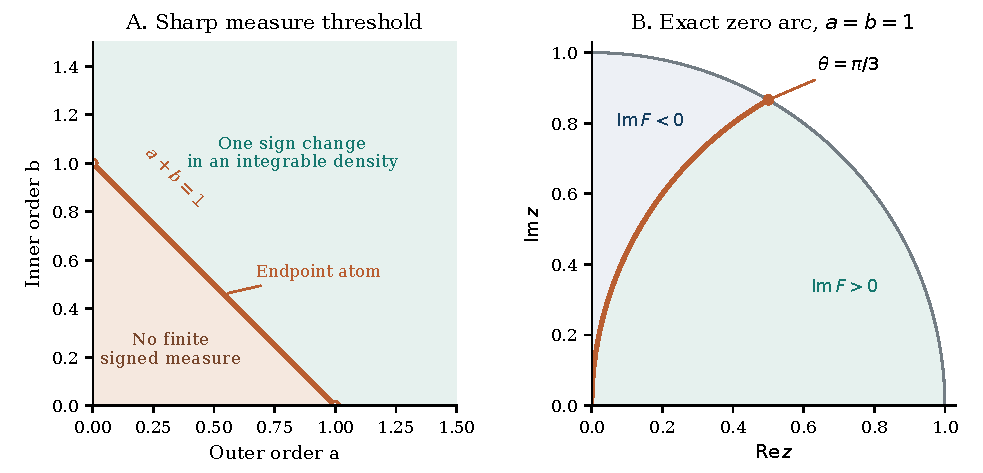
\includegraphics[width=\textwidth]{../figures/measure_geometry.pdf}
\caption{The sharp measure domain for positive real orders (left), and
an exact illustration of the angular-zero theorem in the first quadrant
at $a=b=1$ (right). The separating arc is $|1-z|=1$ and meets the
unit circle at angle $\pi/3$. The phase diagram is a theorem, and the
circular arc is evaluated exactly.}
\label{real:fig:geometry}
\end{figure}

\begin{corollary}[Continuous outer-order motion of the density crossing]
\label{real:cor:order-motion}
Fix $b>0$. If $a_2>a_1>0$ and $a_1+b>1$, then
$r_{a_2,b}<r_{a_1,b}$.
\end{corollary}
\begin{proof}
Put $\delta=a_2-a_1>0$. Multiplication of the moments by
$n^{-\delta}$ and uniqueness in Theorem~\ref{real:thm:measure}
give the Mellin-convolution formula
\[
 k_{a_2,b}(T)=\frac1{\Gamma(\delta)}
   \int_0^T(T-v)^{\delta-1}k_{a_1,b}(v)\,dv.
\]
Absolute exponential integrability justifies convolution and its
Laplace transform. Both sides are continuous for $T>0$, so moment
uniqueness gives pointwise equality. At the old logarithmic crossing
$T_1=-\log r_{a_1,b}$ the integrand is positive almost everywhere.
The new density is therefore positive at $T_1$, and its unique
crossing occurs at $T_2>T_1$. Returning to $r=e^{-T}$ proves the
claim.
\end{proof}

\subsection{Verification and the limits of the geometric conclusion}

The diagnostic program \path{code/geometry_diagnostics.py} and its
output \path{data/geometry_diagnostics.json} accompany these proofs.
They compare two kernel quadratures at nine points; locate four density
crossings, including $(a,b)=(0.5005,0.5)$ near the critical line; check
fifteen strictly negative critical-density values; and compute sixteen
interior-disk zero locations. The exact arc in
Example~\ref{real:ex:circle} supplies an independent comparator.
Twelve additional samples check the critical deficit and its first
four signed derivatives. All diagnostic assertions pass. The checks
are numerical and are not interval certificates; the existence,
uniqueness, and sign assertions rest on the analytic arguments above.

Near the critical line, direct subtraction of the two pieces of the
kernel can be unstable. For $0<a,b<1$ the evaluator instead uses
\[
 I(T)=q_T(1)\int_0^\infty c(s)\,ds
       +\int_0^\infty c(s)\bigl[q_T(s)-q_T(1)\bigr]\,ds,\qquad
 c(s)=g(s)/s.
\]
The first integral is the exact beta expression
\eqref{real:eq:beta}; the second integrand is negative on both
sides of $s=1$. At $a+b=1$ the beta term vanishes exactly. This is
the cancellation used in the proof, translated into a stable evaluator.

Three distinctions delimit the result. First,
$x_{a,b}'(R^2)>0$ does not by itself imply
$\theta_{a,b}'(R)<0$; that stronger angular monotonicity is not proved
here. Second, the monotone motion of the \emph{density} crossing with
$a$ does not imply monotone motion of the angular zero with $a$ or
$b$. Third, when $a+b<1$ the finite signed-measure method is
impossible by Theorem~\ref{real:thm:measure}, but this does not settle
zero uniqueness by other methods. The next section quantifies concentration into the endpoint atom
for fixed $b\in(0,1)$, providing a scale for uniform numerical evaluation.
